\chapter{Methodology}
\label{chap:methodology}

\lettrine[lines=3, findent=3pt, nindent=0pt]{I}{n} this chapter \textcolor{dimgray}{\lipsum[1]}

%----------------------------------------------------
% LAB ENVIRONMENT
%----------------------------------------------------

\section{Lab Environment}
\label{sec:environment}

\textcolor{dimgray}{\lipsum[1]}

%----------------------------------------------------
% TECHNICAL MODEL
%----------------------------------------------------

\subsection{Technical Model}
\label{subsec:technical-model}

\textcolor{dimgray}{\lipsum[1]}

%----------------------------------------------------
% IMPLEMENTATION
%----------------------------------------------------

\section{Implementation}
\label{sec:implemntation}

\textcolor{dimgray}{\lipsum[1]}

%----------------------------------------------------
% CLASSIFIER
%----------------------------------------------------

\subsection{Anomaly Classifier}
\label{subsec:classifier-implementation}

\textcolor{dimgray}{\lipsum[1]}

%----------------------------------------------------
% PREPROCESSING
%----------------------------------------------------

\subsubsection{Dataset Preprocessing}
\label{subsubsec:ac-preprocessing}

\begin{figure}[h!]
    \centering
    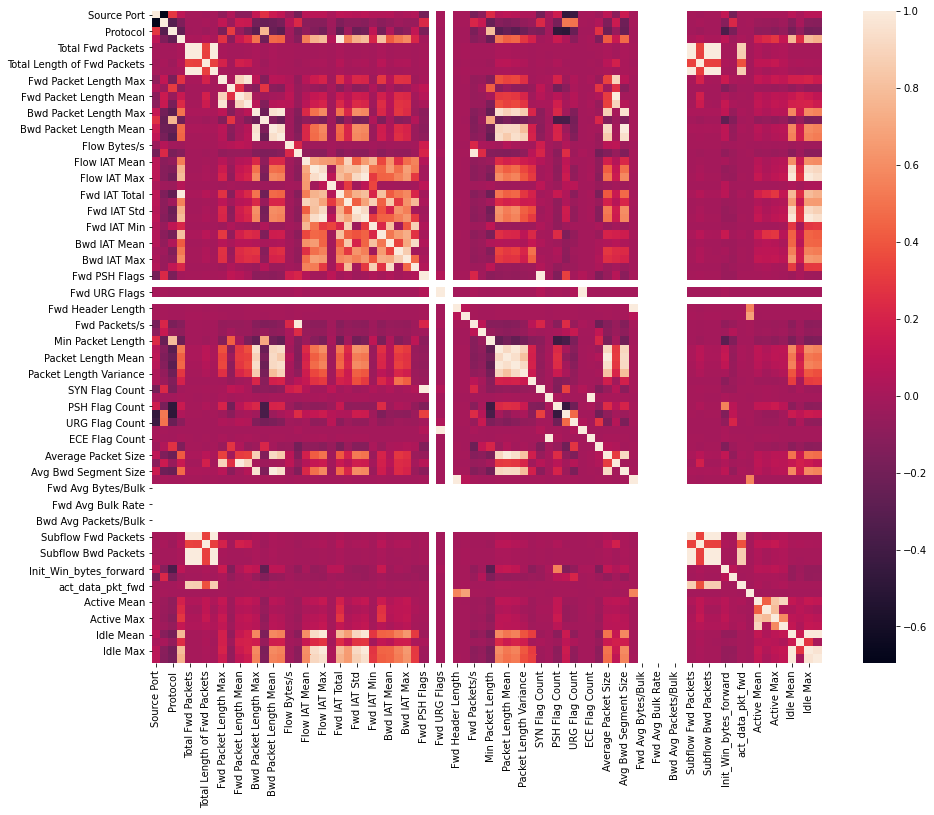
\includegraphics[scale=0.5]{assets/figures/chapter3/feature-correlation.png}
    \caption{Feature Correlation Matrix of CICIDS2017}
    \label{fig:feature-correlation}
\end{figure}

%----------------------------------------------------
% CLASSIFICATION
%----------------------------------------------------

\subsubsection{Classification}
\label{subsubsec:ac-classification}

\textcolor{dimgray}{\lipsum[1]}

\begin{figure}[h!]
    \centering
    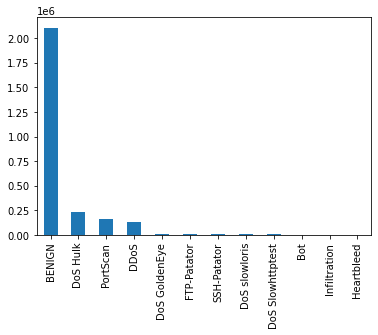
\includegraphics[scale=0.6]{assets/figures/chapter3/traffic_distribution.png}
    \caption{Traffic Distribution}
    \label{fig:traffic-distribution}
\end{figure}

%----------------------------------------------------
% NETWORK MONITOR
%----------------------------------------------------

\subsection{Network Monitor}
\label{subsec:monitor-implementation}

\textcolor{dimgray}{\lipsum[1]}

%----------------------------------------------------
% FLOW IDENTIFICATION
%----------------------------------------------------

\subsubsection{Flow Identification}
\label{subsubsec:nm-flow-id}

\textcolor{dimgray}{\lipsum[1]}

\begin{code}[colback=white]{Monitor.py}
if packet.getFwdID() in current_flows.keys():
flow = current_flows[packet.getFwdID()]

# check for timeout
# for some reason they only do it if packet count > 1
if (packet.getTimestamp() - flow.getFlowStartTime()) > FlowTimeout:
    classify(flow.terminated())
    del current_flows[packet.getFwdID()]
    flow = Flow(packet)
    current_flows[packet.getFwdID()] = flow

# check for fin flag
elif packet.getFINFlag() or packet.getRSTFlag():
    flow.new(packet, 'fwd')
    classify(flow.terminated())
    del current_flows[packet.getFwdID()]
    del flow
\end{code}

\textcolor{dimgray}{\lipsum[1]}

%----------------------------------------------------
% FEATURE EXTRACTION
%----------------------------------------------------

\subsubsection{Flow Feature Extraction}
\label{subsubsec:nm-flow-extraction}

%----------------------------------------------------
% INTRUSION DETECTION SYSTEM
%----------------------------------------------------

\subsection{Intrusion Detection System}
\label{subsec:ids-implementation}

%----------------------------------------------------
% EVALUATION
%----------------------------------------------------

\section{Evaluation}
\label{sec:evaluation}

\textcolor{dimgray}{\lipsum[1-15]}

%----------------------------------------------------
% ATTACK SIMULATION
%----------------------------------------------------

\subsection{Attack Simulation}
\label{subsec:attack-simulation}

\textcolor{dimgray}{\lipsum[1-20]}
